\begin{frame}{任务 (Job) 的数学模型}

    \begin{columns}

        \column{0.5\textwidth}

        固有属性:

        \begin{itemize}
            \item $J_c$ 任务需要的计算核心数
            \item $J_m$ 任务需要的内存大小
            \item $J_t$ 任务的类型 (Moldable/Rigid)
        \end{itemize}

        \column{0.5\textwidth}

        状态属性:

        \begin{itemize}
            \item $J_l$ 任务长度(小时)
            \item $t_a$ 任务到达时刻 (arrival time)
            \item $J_r$ 任务上一次执行所在的区域
        \end{itemize}

    \end{columns}

\end{frame}

\begin{frame}{Downey 加速模型}

    并行度 (parallelism) 具有均值 $A$ 和标准差 $\sigma$ 两个参数.

    将 $0 \leqslant \sigma \leqslant 1$ 的模型称为Low variance model, 将 $\sigma > 1$ 的模型称为High variance model.

    \begin{columns}

        \column{0.5\textwidth}

        \begin{figure}
            \centering
            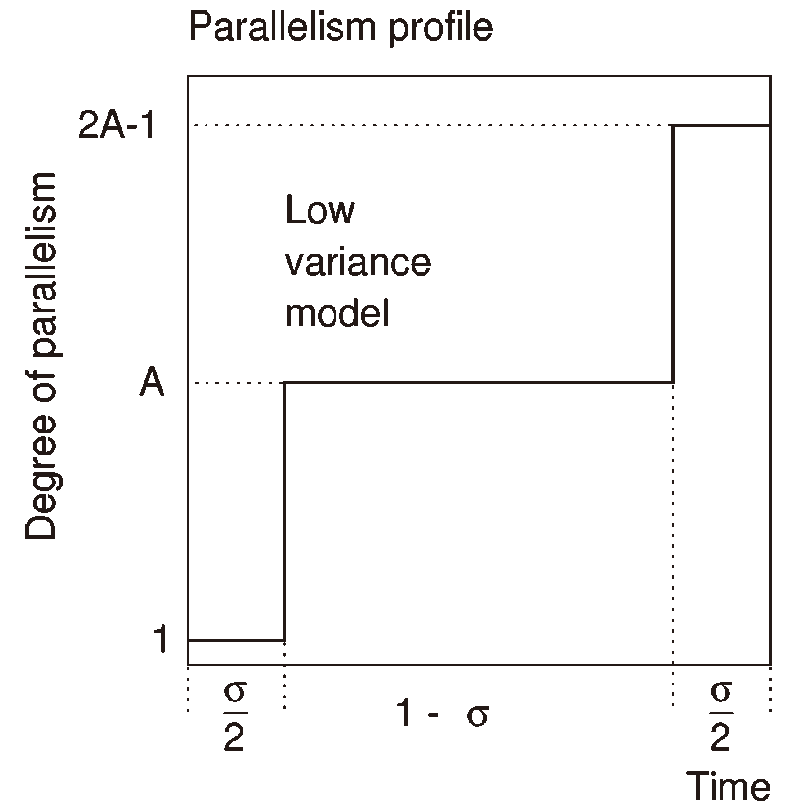
\includegraphics[scale=0.15]{pics/low_variance_model.png}
            \caption{Low variance model}
        \end{figure}

        \column{0.5\textwidth}

        \begin{figure}
            \centering
            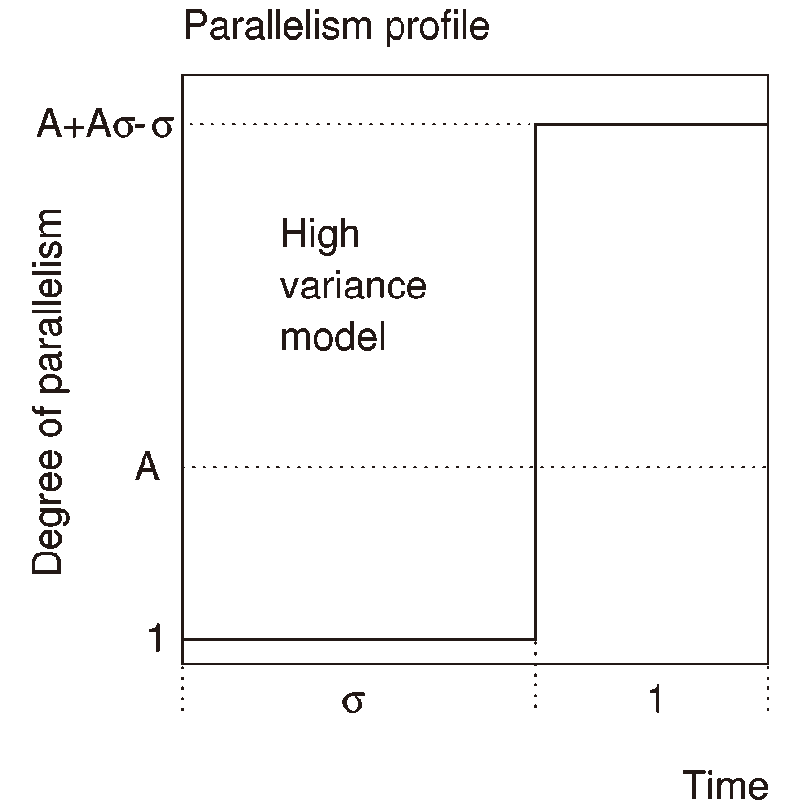
\includegraphics[scale=0.15]{pics/high_variance_model.png}
            \caption{High variance model}
        \end{figure}

    \end{columns}

\end{frame}

\begin{frame}{Downey 加速模型}{加速系数 $SU(n)$ 的计算}

    \begin{columns}

        \column{0.6\textwidth}

        当 $0 \leqslant \sigma \leqslant 1$ 时:

        \begin{equation*}
            SU(n)= \begin{cases}
                \frac{A n}{A + \sigma(n-1) / 2},                 & 1 \leqslant n \leqslant A, \\
                \frac{A n}{\sigma(A-1 / 2) + n(1 - \sigma / 2)}, & A < n \leqslant 2 A-1,     \\
                A,                                               & n > 2A - 1 .
            \end{cases}
        \end{equation*}

        当 $\sigma > 1$ 时:

        \begin{equation*}
            SU(n)= \begin{cases}
                \frac{n A(\sigma + 1)}{A + A \sigma - \sigma + n \sigma}, & 1 \leqslant n \leqslant A + A \sigma - \sigma, \\
                A,                                                        & n > A + A \sigma - \sigma .
            \end{cases}
        \end{equation*}

        其中 $n$ 为计算核心数.

        \column{0.4\textwidth}

        \begin{figure}
            \centering
            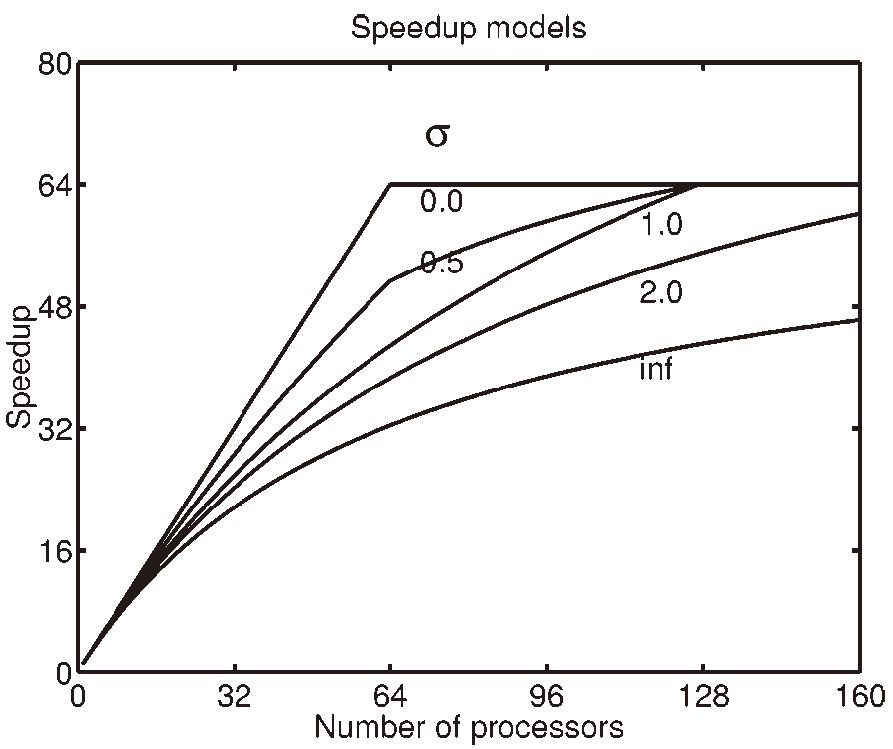
\includegraphics[scale=0.17]{pics/speedup_curve.png}
            \caption{Speedup curves for a range of values of $\sigma$ when $A = 64$}
        \end{figure}
    \end{columns}
\end{frame}

\begin{frame}[fragile]{任务类型 $J_t$ 与实际执行时间 $T^e$}{Moldable/Rigid}

    任务类型 $J_t$ 影响任务实际执行时间 $T^e$ 的计算.

    \centering
    \begin{minipage}{0.7\textwidth}
        \IncMargin{1.5em}
        \begin{algorithm}[H]
            \SetAlgoLined
            \caption{计算任务实际执行时间 $T^e$}
            \If{$J_t =$ Moldable}{$T^e = J_l \cdot \frac{SU(J_c)}{SU(I_c)}$\;}
            \If{$J_t =$ Rigid}{\eIf{$J_c \leqslant I_c$}{$T^e = J_l$\;}{任务调度失败\;}}
        \end{algorithm}
        \DecMargin{1.5em}
    \end{minipage}

\end{frame}

\begin{frame}{挂起时间 $T_w$ 与恢复时间 $T_l$}

    当正在执行任务的实例到期时, 任务需要挂起到硬盘, 该操作需要的时间为:

    \begin{equation*}
        T_w = \frac{J_m}{v_w}
    \end{equation*}

    当任务首次在实例中运行或从挂起状态恢复时, 任务需要加载到内存, 该操作需要的时间为:

    \begin{equation*}
        T_l = \begin{cases}
            \dfrac{J_m}{v_l},          & J_r = None \, \text{or} \, J_r = I_r, \\
            2 \times \dfrac{J_m}{v_l}, & \text{otherwise}.
        \end{cases}
    \end{equation*}

\end{frame}
